\subsection{Multiple Entities}

\subsection{Spawning Entities at Runtime}

\subsection{Video feed} \label{06:VideoFeed}

\begin{figure}[h]
    \centering
    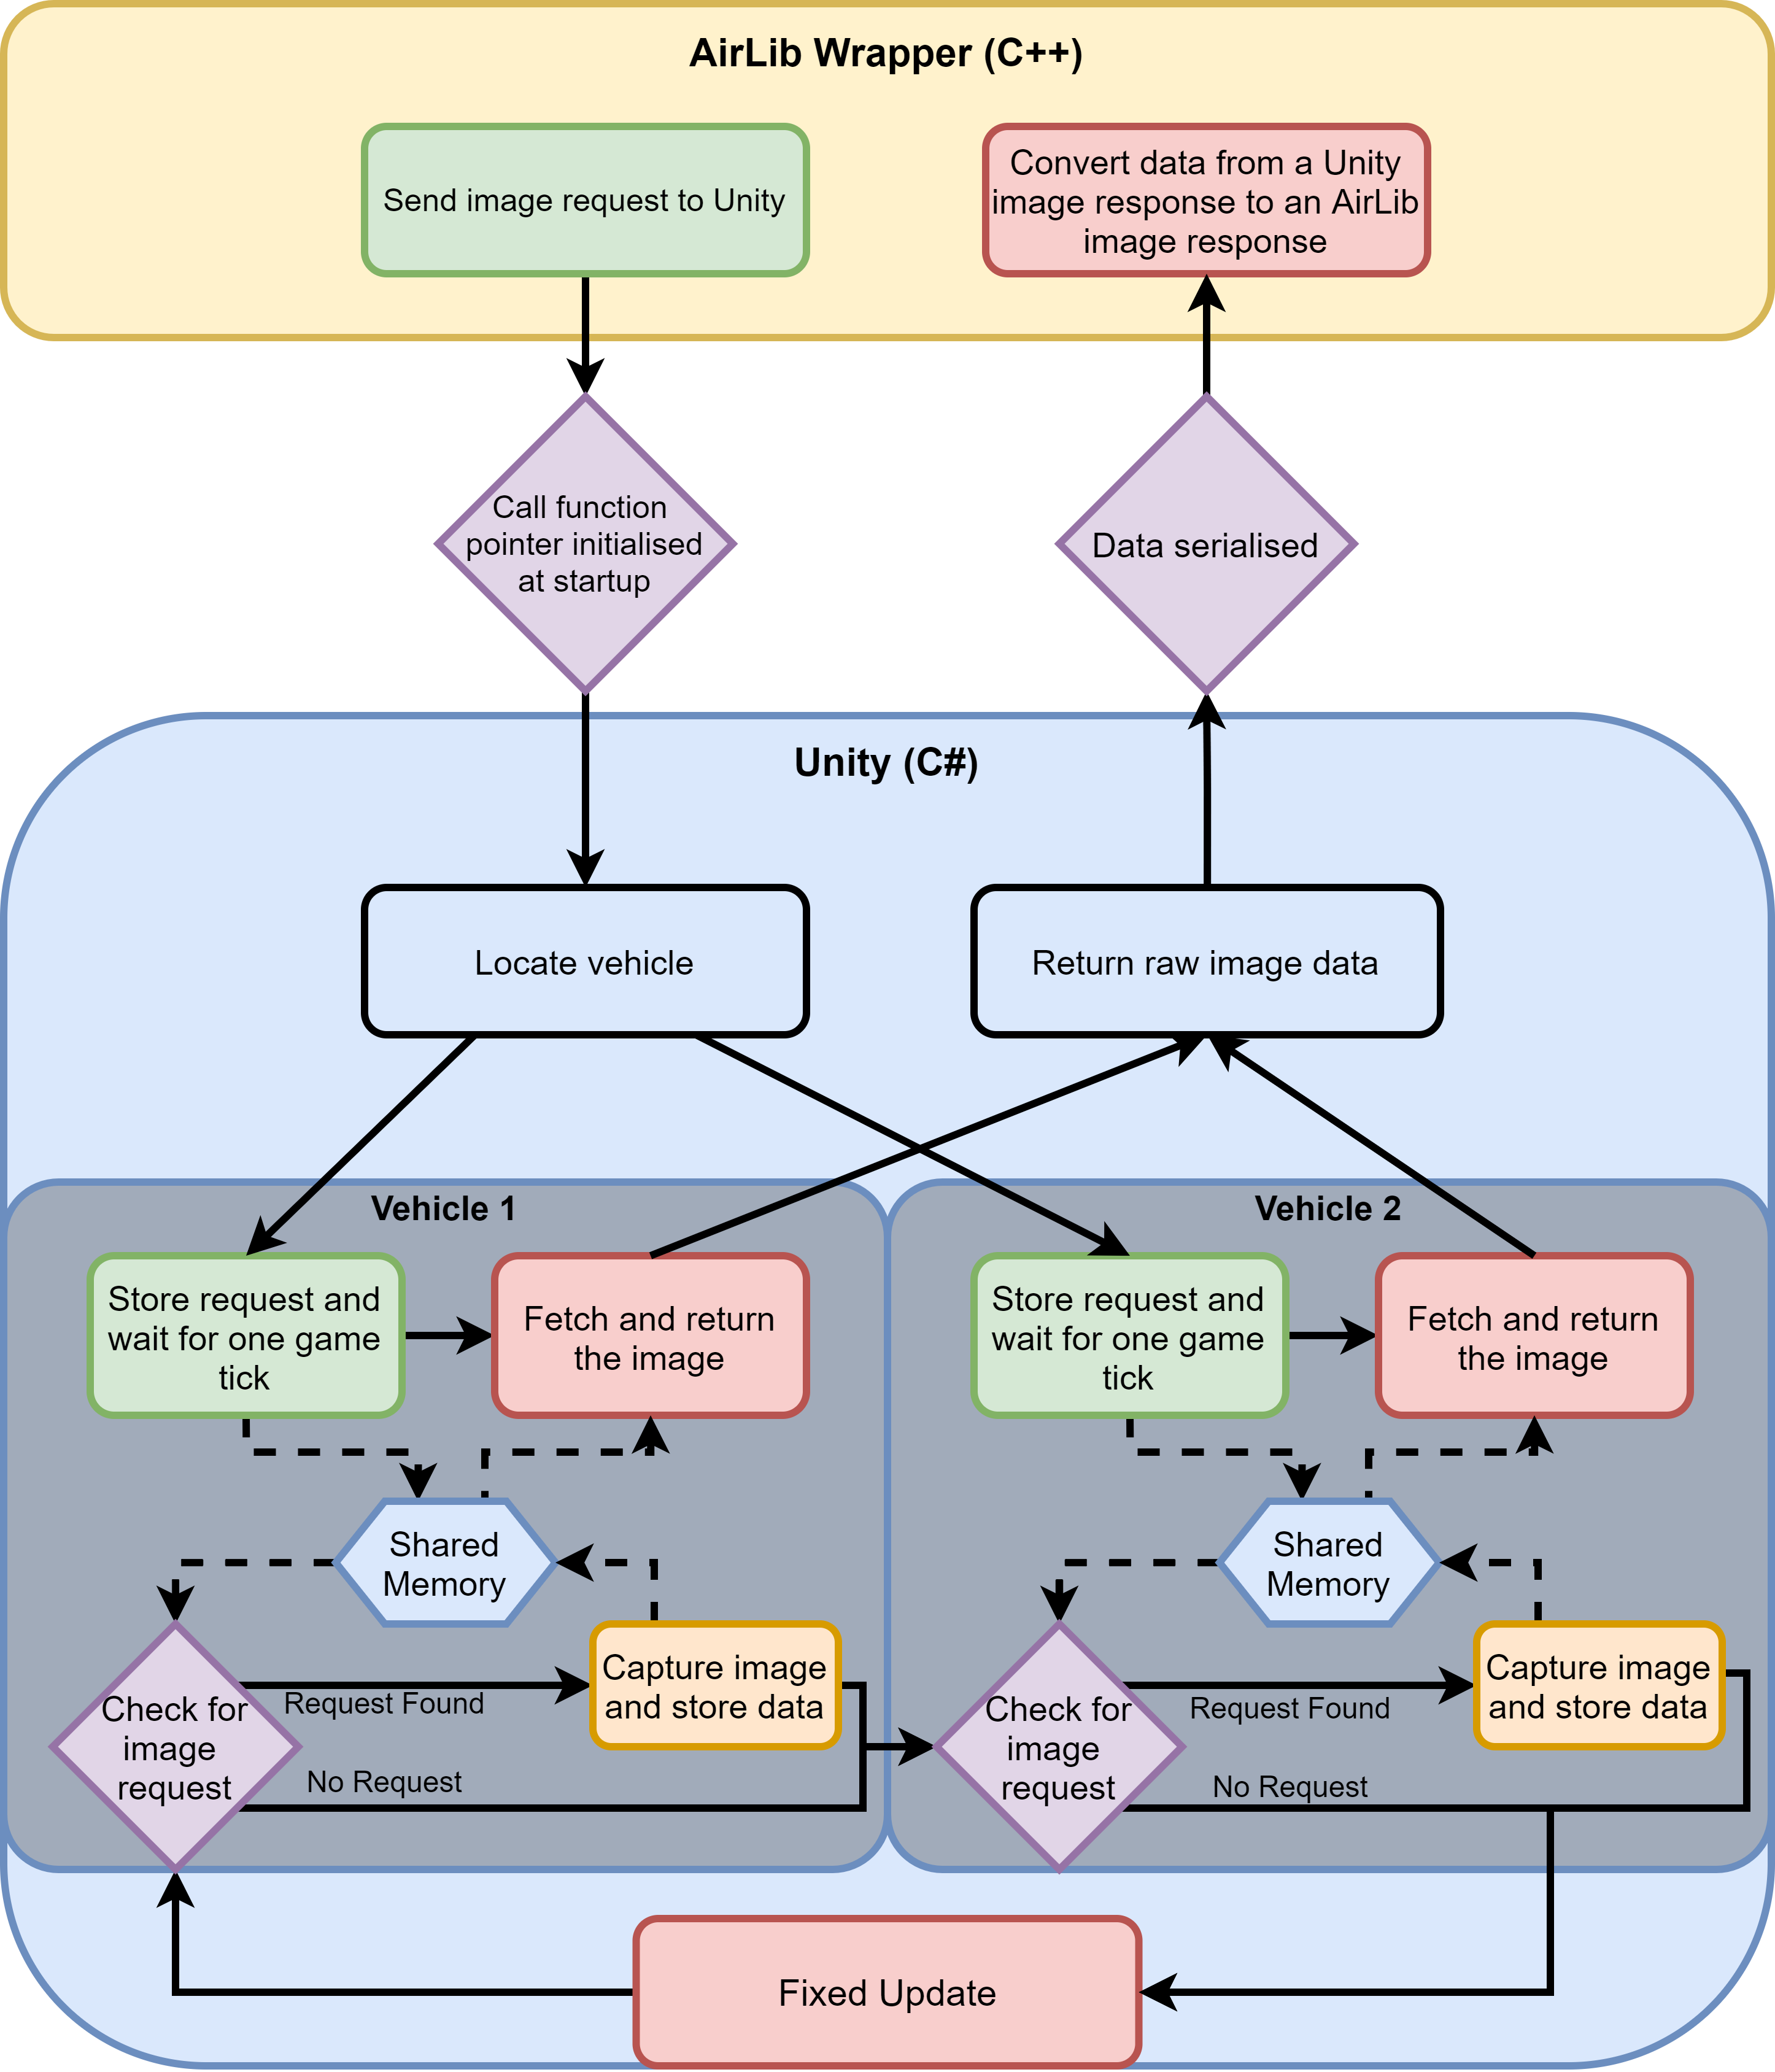
\includegraphics[width=1.0\textwidth]{06_Implementation/00_AirSim/Diagrams/imagecapture.png}
    \caption{} \label{06:imageCapture}
\end{figure}

\begin{figure}[h]
    \centering
    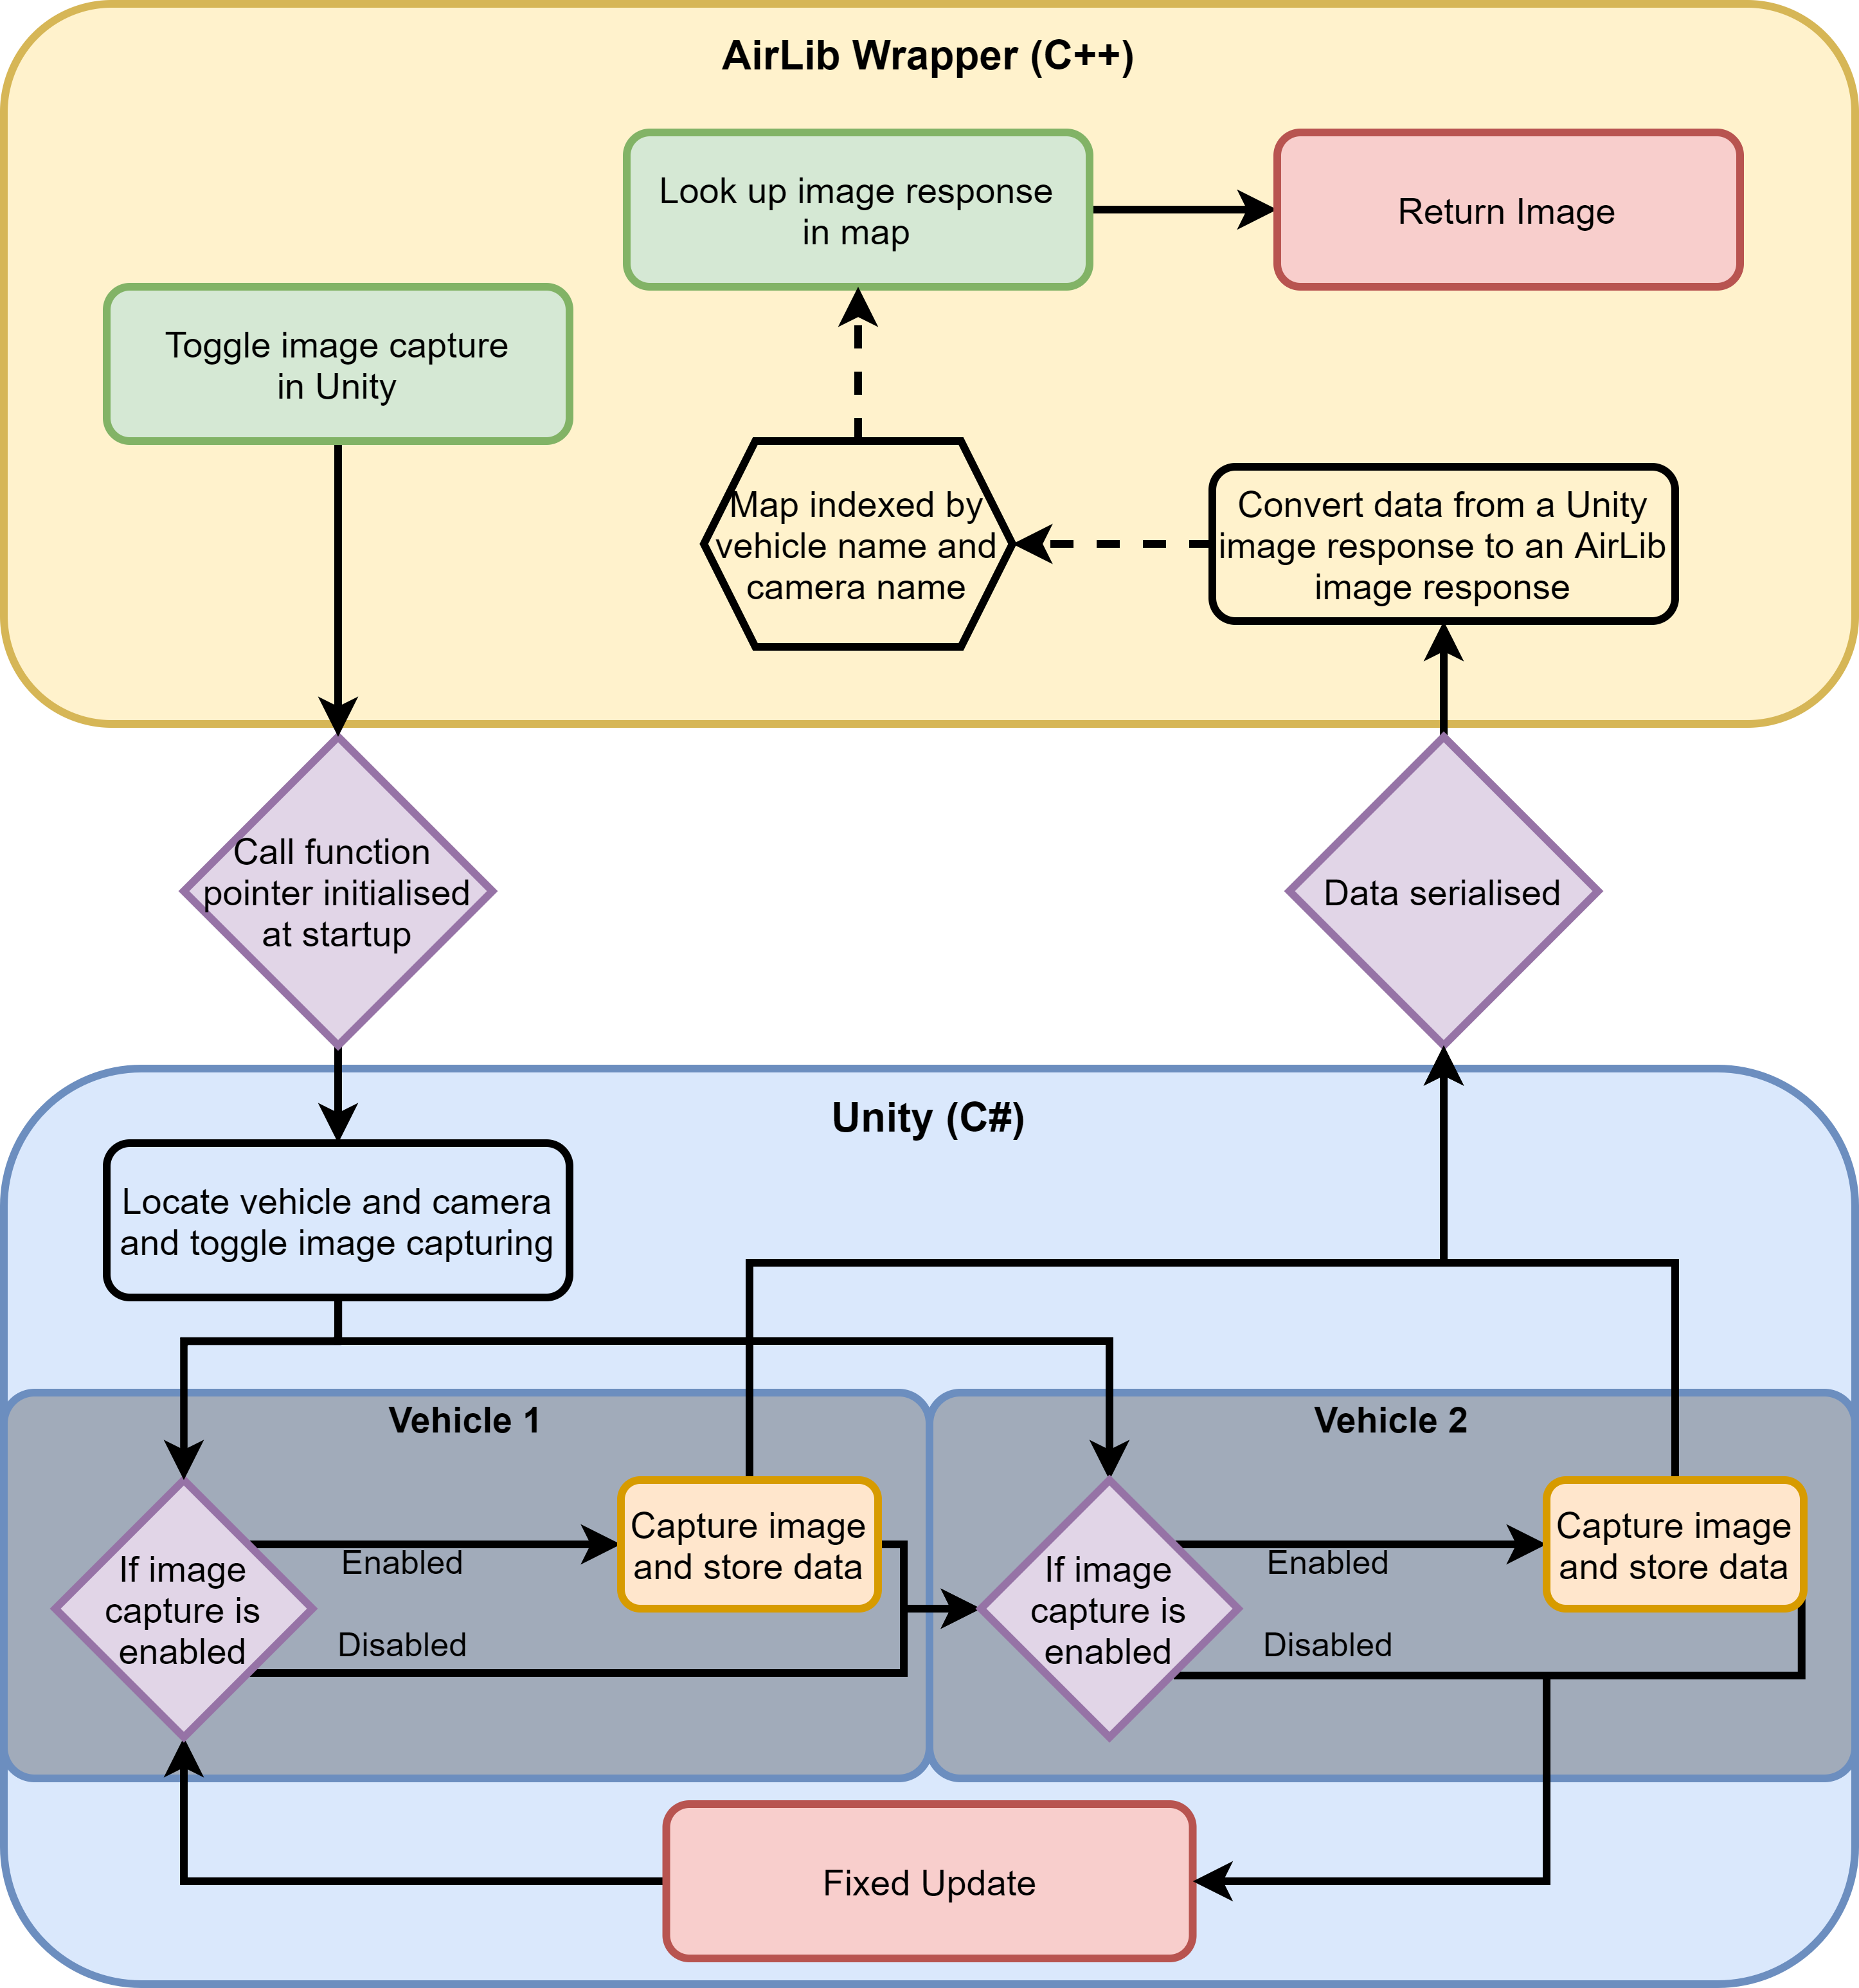
\includegraphics[width=1.0\textwidth]{06_Implementation/00_AirSim/Diagrams/imagecaptureUpdated.png}
    \caption{} \label{06:imageCaptureUpdated}
\end{figure}

\subsection{Adding Pedestrians}

\subsection{Additional APIs}

\begin{figure}[h]
    \centering
    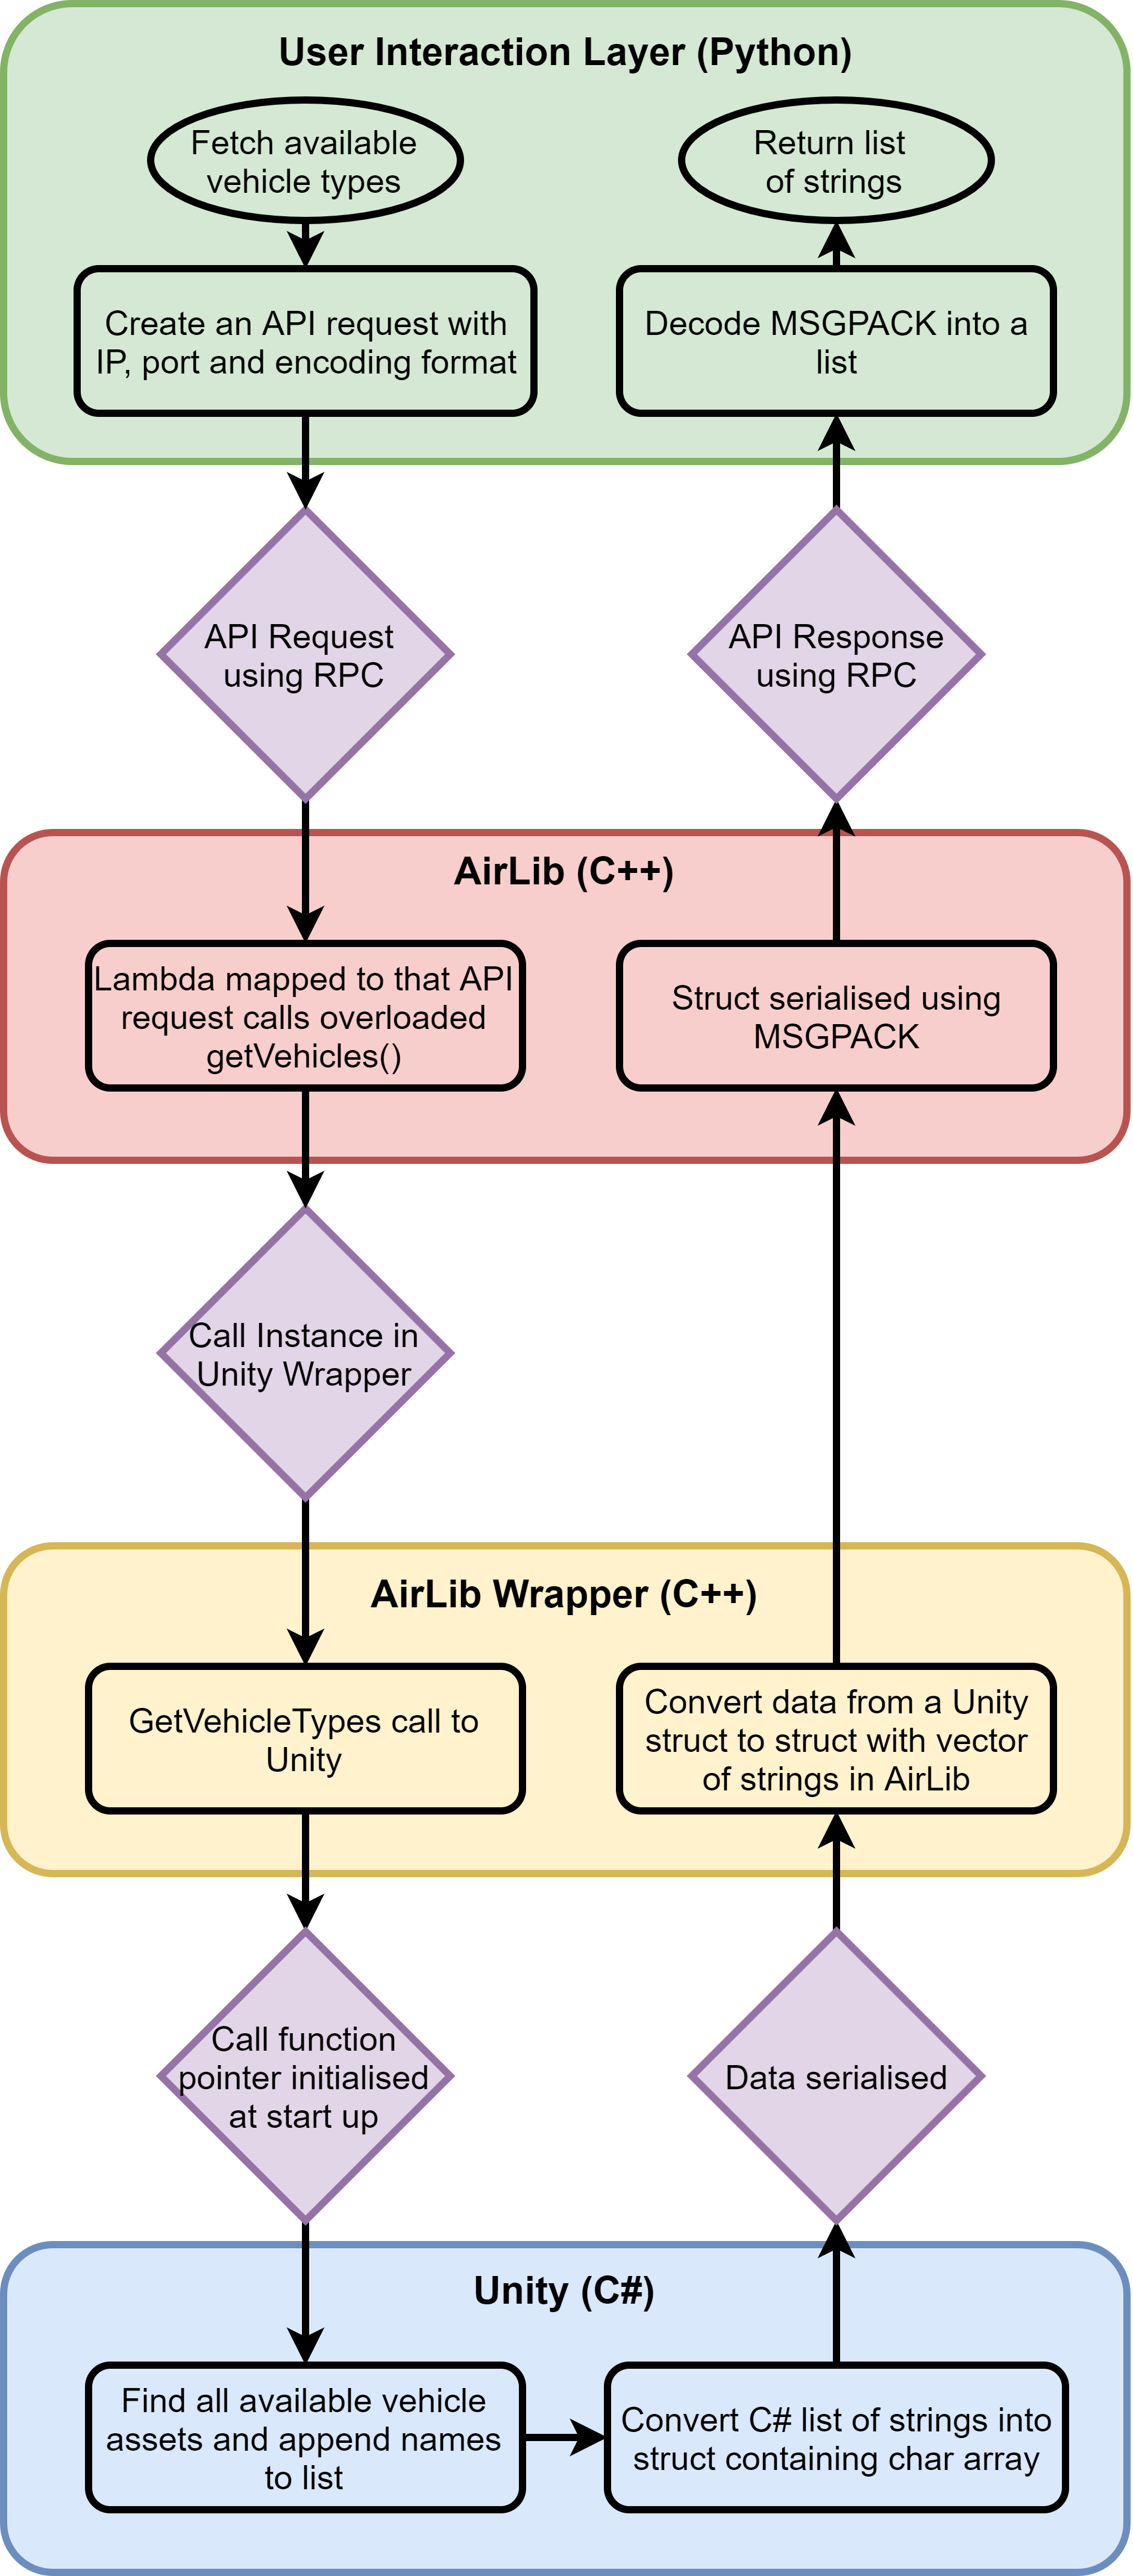
\includegraphics[width=0.6\textwidth]{06_Implementation/00_AirSim/Diagrams/stringArray.png}
    \caption{High-level overview of the API that fetches available vehicle types. For APIs that require arguments, these will be encoded and added to the API request. The main change between different API requests is what happens in Unity.} \label{06:stringList}
\end{figure}

\subsection{Minor Features added}
%freecam and change between vehicles and entities